\documentclass[border=2mm]{standalone}
\usepackage{pgfplots}
\pgfplotsset{compat=1.18}
\usetikzlibrary{arrows.meta,
  calc,
  positioning,
  decorations.pathreplacing,
  calligraphy}
\usepackage{xcolor}
\definecolor{den-1}{HTML}{111111}   % Đen #111111
\definecolor{den-2}{HTML}{222222}   % Đen #222222
\definecolor{den-3}{HTML}{333333}   % Đen #333333
\definecolor{den-4}{HTML}{444444}   % Đen #444444
\definecolor{den-5}{HTML}{555555}   % Đen #555555
\definecolor{den-6}{HTML}{666666}   % Đen #666666
\definecolor{do-1}{HTML}{440000}   % Đỏ #440000 trầm hơn, hợp với đen #111111
\definecolor{do-2}{HTML}{660000}   % Đỏ #660000 sẫm, hợp với đen #222222
\definecolor{do-3}{HTML}{880000}   % Đỏ #880000 đậm vừa, hợp với đen #333333
\definecolor{do-4}{HTML}{AA0000}   % Đỏ #AA0000 tươi vừa, hợp với đen #444444
\definecolor{do-5}{HTML}{CC0000}   % Đỏ #CC0000 tươi hơn, hợp với đen #555555
\definecolor{do-6}{HTML}{EE0000}   % Đỏ #EE0000 sáng hơn, hợp với đen #666666
% Thiết lập vị trí đặt nhãn gốc tọa độ
\tikzset{
  >=Stealth,
  originlabel/.style={
    font=\small\sf,
    anchor=north east, % Vị trí tương đối so với gốc
    yshift=-0.1ex,     % Điều chỉnh vị trí dọc một chút
    xshift=-0.1ex      % Điều chỉnh vị trí ngang một chút
  }
}
\begin{document}
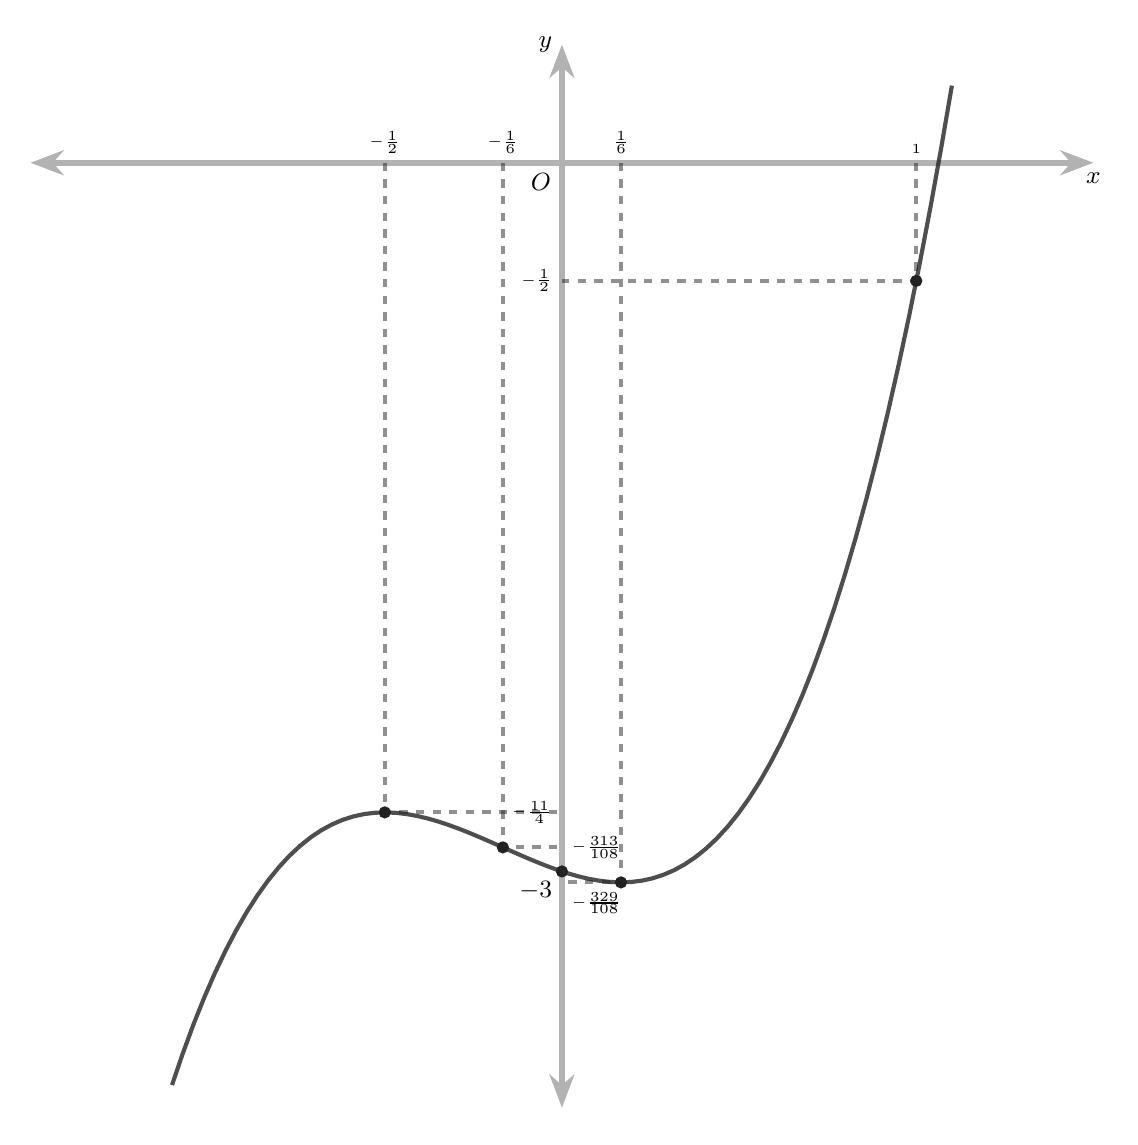
\begin{tikzpicture}
  \begin{axis}[
    font=\small\sf,
    axis lines = middle,
    axis line style={<->, line width=2pt, color=den-6!50},
    xlabel=$x$, ylabel=$y$,
    xlabel style={below, font=\small\sf},
    ylabel style={left, font=\small\sf},
    xmin=-1.5, xmax=1.5,
    ymin=-4, ymax=.5,
    scale only axis,
    height=13.5cm,
    width=13.5cm,
    xtick={},
    xticklabels={},
    xtick style={draw=none},
    ytick={},    
    yticklabels={},
    ytick style={draw=none},  
    tick label style={font=\footnotesize\sf},
    clip=false,
  ]
    \node[originlabel] at (axis cs:0,0) {$O$};

    \addplot[dashed, line width=1.5pt, color=den-2, opacity=.5] coordinates {
        (-1/2,0)
        (-1/2,-11/4)
        (0,-11/4)
        };
    \node at (-1/2,0) [above] {\tiny $-\frac{1}{2}$};
    \node at (0,-11/4) [left] {\tiny $-\frac{11}{4}$};

    \addplot[dashed, line width=1.5pt, color=den-2, opacity=.5] coordinates {
        (-1/6,0)
        (-1/6,-313/108)
        (0,-313/108)
        };
    \node at (-1/6,0) [above] {\tiny $-\frac{1}{6}$};
    \node at (0,-313/108) [right] {\tiny $-\frac{313}{108}$};

    \addplot[dashed, line width=1.5pt, color=den-2, opacity=.5] coordinates {
        (1/6,0)
        (1/6,-329/108)
        (0,-329/108)
        };
    \node at (1/6,0) [above] {\tiny $\frac{1}{6}$};
    \node at (0,-329/108) [below right] {\tiny $-\frac{329}{108}$};

    \node at (0,-3) [below left] {$-3$};

    \addplot[dashed, line width=1.5pt, color=den-2, opacity=.5] coordinates {
        (1,0)
        (1,-1/2)
        (0,-1/2)
        };
    \node at (1,0) [above] {\tiny $1$};
    \node at (0,-1/2) [left] {\tiny $-\frac{1}{2}$};
    
    \addplot[
      domain=-3:3,
      restrict y to domain=-4:.5,
      samples=200,
      line width=1.5pt,
      color=den-2,
      opacity=.8
      ]
        {2*x^3+x^2-(1/2)*x-3};
        
    \addplot[only marks, mark=*, mark size=2pt, color=den-2] coordinates {
        (0,-3)
        (-1/2,-11/4)
        (1/6,-329/108)
        (-1/6,-313/108)
        (1,-1/2)
        };
  \end{axis}
\end{tikzpicture}
\end{document}